\chapter{Diagram dan \textit{Pseudocode} Algoritma}

\begin{figure}[H]
	\centering
	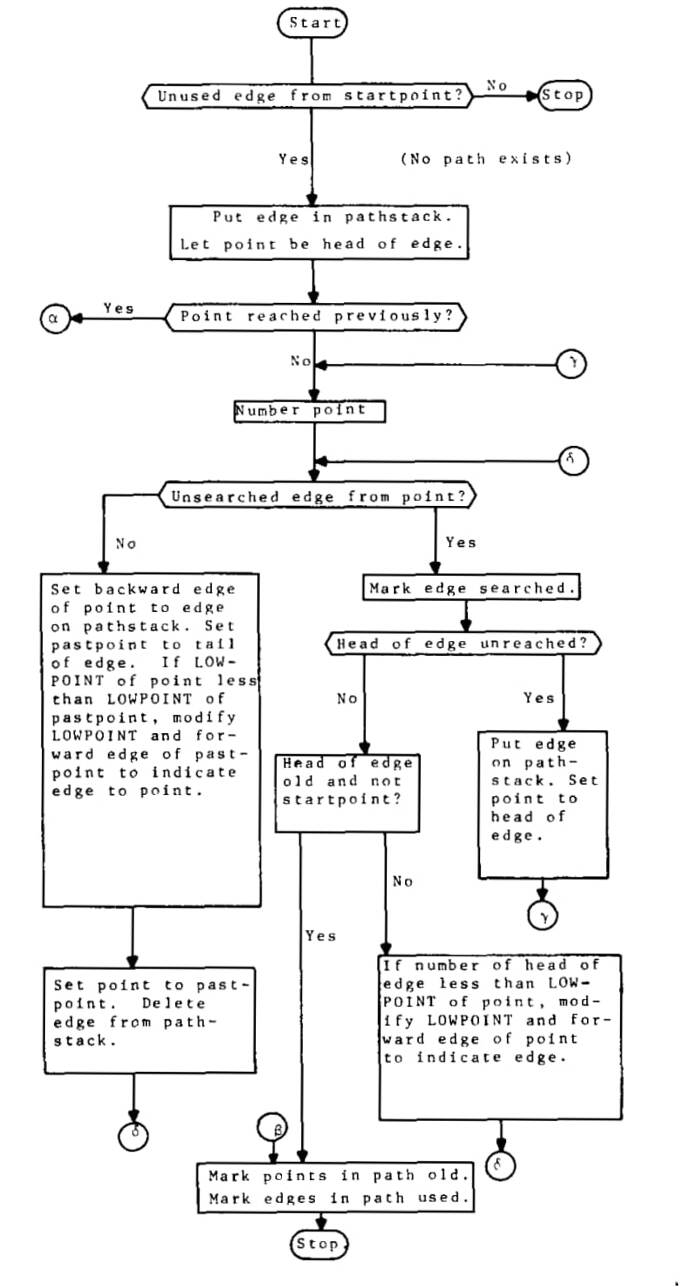
\includegraphics[width=0.7\textwidth]{chapter-3/path-finding-hopcroft.jpeg}
	\caption{Algoritma \ac{DFS} untuk \textit{pathfinding} \parencite{hopcroft1973algorithm}}
	\label{fig:hopcroft-dfs}
\end{figure}

\begin{algorithm}
	\makeatletter
	\renewcommand{\ALG@name}{Algoritma}
	\makeatother
	\caption{Prim \textit{Generator} Labirin}\label{alg:prim}
	\renewcommand{\algorithmicrequire}{\textbf{Masukan:}}
	\renewcommand{\algorithmicensure}{\textbf{Keluaran:}}
	\begin{algorithmic}[1]
		\Require $labirin$ dan $dimensi$
		\Ensure $labirin$ yang telah terbangun
		\State Inisialisasi $labirin$ penuh dengan halangan
		\State Buat halangan pertama jadi sel kosong
		\State Tambah semua halangan, disamping sel kosong, ke $list\_halangan$
		\While{$list\_halangan$ belum kosong}
		\State $halangan\_kini$ $\gets$ halangan acak di $list\_halangan$
		\If{$halangan\_kini$ hanya punya satu sel kosong didekatnya}
		\State Ubah $halangan\_kini$ menjadi sel kosong
		\State Masukkan halangan di sekitar $halangan\_kini$ ke $list\_halangan$
		\EndIf
		\State hapus $halangan\_kini$ dari $list\_halangan$
		\EndWhile
	\end{algorithmic}
\end{algorithm}


\begin{algorithm}
	\makeatletter
	\renewcommand{\ALG@name}{Algoritma}
	\makeatother
	\caption{\ac{DFS} pada labirin}\label{alg:dfs-sw}
	\renewcommand{\algorithmicrequire}{\textbf{Masukan:}}
	\renewcommand{\algorithmicensure}{\textbf{Keluaran:}}
	\begin{algorithmic}[1]
		\Require $baris$, $kolom$, dan $memori$
		\Ensure $langkah\_diambil$
		\State $memori \gets$ [$baris$,$kolom$]
		\If{[$baris$,$kolom$] = tujuan}
		\State return 0 \EndIf
		\State $langkah\_diambil$ $\gets$ NULL
		\For{$aksi$ dari [$gerak\_atas$, $gerak\_bawah$, $gerak\_kiri$, $gerak\_kanan$]}
		\State $kolom\_baru$, $baris\_baru$ $\gets$ lingkungan($aksi$, $kolom$, $baris$)
		\If{[$kolom\_baru$,$baris\_baru$] \textbf{tidak di} $memori$}
		\State $langkah\_DFS$ $\gets$ DFS($kolom\_baru$, $baris\_baru$, $memori$) + 1
		\If{$langkah\_diambil$ = NULL \textbf{or} $langkah\_diambil < langkah\_DFS$}
		\State $langkah\_diambil \gets langkah\_DFS$
		\EndIf
		\EndIf
		\EndFor
		\State return $langkah\_diambil$
	\end{algorithmic}
\end{algorithm}

\begin{algorithm}
	\makeatletter
	\renewcommand{\ALG@name}{Algoritma}
	\makeatother
	\caption{\ac{RL} menggunakan \textit{Q-Learning} diadaptasi dari \parencite{sutisna2023faraneq}}\label{alg:rl-qlearning}
	\renewcommand{\algorithmicrequire}{\textbf{Masukan:}}
	\renewcommand{\algorithmicensure}{\textbf{Keluaran:}}
	\begin{algorithmic}[1]
		\Require jumlah episode, \textit{learning rate ($\alpha$)}, dan \textit{discount factor ($\gamma$)}
		\Ensure \textit{Q-Table}
		\State Inisialisasi \textit{Q-Table} untuk setiap \textit{state} dan aksi
		\While{$banyak\_episode < jumlah\_episode$}
		\State $s_{t} \gets s_0$
		\While{$s_t \neq s_{terminal}$}
		\State Pilih aksi ($A$) untuk \textit{state} kini ($s_t$)
		\State Lakukan $A$, dapatkan \textit{reward} dan $s_{t+1}$ \label{algline:q-reward}
		\State Hitung nilai Q-Table indeks terkini \Comment{dengan Persamaan \ref{eq:q-learning}}
		\State $s_t \gets s_{t+1}$
		\EndWhile
		\State $banyak\_episode \gets banyak\_episode + 1$
		\EndWhile
	\end{algorithmic}
\end{algorithm}

\begin{algorithm}
	\makeatletter
	\renewcommand{\ALG@name}{Algoritma}
	\makeatother
	\caption{Desain fungsi \textit{reward}}\label{alg:rl-reward-function}
	\renewcommand{\algorithmicrequire}{\textbf{Masukan:}}
	\renewcommand{\algorithmicensure}{\textbf{Keluaran:}}
	\begin{algorithmic}[1]
		\Require $baris$, $kolom$, $memori$, dan aksi
		\Ensure $reward$
		\State $kolom\_baru$, $baris\_baru$ $\gets$ lingkungan($aksi$, $kolom$, $baris$)
		\If{[$kolom\_baru$,$baris$] = halangan} \label{algline:reward-c1}
		\State return $C_1$
		\EndIf
		\If{[$kolom\_baru$,$baris$] \textbf{ada di} $memori$} \label{algline:reward-c2}
		\State return $C_2$
		\EndIf
		\If{[$kolom\_baru$,$baris$] = tujuan} \label{algline:reward-c3}
		\State return $C_3$
		\EndIf
		\State return $C_4$ \label{algline:reward-c4}
	\end{algorithmic}
\end{algorithm}

\begin{algorithm}
	\makeatletter
	\renewcommand{\ALG@name}{Algoritma}
	\makeatother
	\caption{Ekstensi algoritma \ac{RL} dengan memoisasi pintar adopsi dari \parencite{mazaya2024reinforcement}}\label{alg:rl-qmemo}
	\renewcommand{\algorithmicrequire}{\textbf{Masukan:}}
	\renewcommand{\algorithmicensure}{\textbf{Keluaran:}}
	\begin{algorithmic}[1]
		\Require jumlah episode, \textit{learning rate} ($\alpha$), dan \textit{discount factor} ($\gamma$)
		\Ensure \textit{Q-Table}
		\State Inisialisasi \textit{Q-Table} untuk setiap \textit{state} dan aksi
		\While{$banyak\_episode < jumlah\_episode$}
		\State $s_{t} \gets s_0$
		\While{$s_t \neq s_{terminal}$}
		\State Pilih aksi ($A$) untuk \textit{state} kini ($s_t$)
		\State Lakukan $A$, dapatkan \textit{reward} dan $s_{t+1}$
		\State Hitung nilai Q-Table indeks terkini \Comment{dengan Persamaan \ref{eq:q-learning}}
		\State $s_t \gets s_{t+1}$
		\EndWhile
		\State $banyak\_episode \gets banyak\_episode + 1$
		\State $cr_t$ $\gets$ \textit{cumulative reward} dari \textit{Q-Table}
		\If{$cr_t\ >\ cr_{t-1}$}
		\State Ubah nilai $maxQ(s_{t+1},a))$ dari \textit{Q-Table} \label{algline:q-memo-equation} \Comment{dengan Persamaan \ref{eq:q-memo-overwrite}}
		\EndIf
		\State $cr_{t-1} \gets cr_t$
		\State \textit{memori Q-Table} $\gets$ \textit{Q-Table}
		\State $episode \gets episode + 1$
		\EndWhile
	\end{algorithmic}
\end{algorithm}

\begin{algorithm}
	\makeatletter
	\renewcommand{\ALG@name}{Algoritma}
	\makeatother
	\caption{Pembagian HW/SW \textit{co-design}}\label{alg:hw-sw-sep}
	\renewcommand{\algorithmicrequire}{\textbf{Masukan:}}
	\renewcommand{\algorithmicensure}{\textbf{Keluaran:}}
	\begin{algorithmic}[1]
		\Require jumlah episode, \textit{learning rate} ($\alpha$), dan \textit{discount factor} ($\gamma$)
		\Ensure \textit{Q-Table}
		\State \alghighlight{yellow!50}{Inisialisasi \textit{Q-Table} untuk setiap \textit{state} dan aksi \label{algline:initialize-q-table-hw} \Comment{\textbf{Perangkat keras}}}
		\State \alghighlight{yellow!50}{Simpan $\gamma$ dan $\alpha$ pada akselerator \Comment{\textbf{Perangkat keras}}}
		\While{$banyak\_episode < jumlah\_episode$}
		\State $s_{t} \gets s_0$
		\While{$s_t \neq s_{terminal}$}
		\State \alghighlight{yellow!50}{Pilih aksi ($A$) untuk \textit{state} kini ($s_t$) \label{algline:choose-action-hw}  \Comment{\textbf{Perangkat keras}}}
		\State Lakukan $A$, dapatkan \textit{reward} dan $s_{t+1}$
		\State \alghighlight{yellow!50}{Simpan $s_{t+1}$ pada akselerator \Comment{\textbf{Perangkat keras}}}
		\State \alghighlight{yellow!50}{Hitung nilai \textit{Q-Table} indeks terkini \label{algline:q-table-update-hw} \Comment{\textbf{Perangkat keras}}}
		\State $s_t \gets s_{t+1}$
		\EndWhile
		\State $banyak\_episode \gets banyak\_episode + 1$
		\State $cr_t$ $\gets$ \textit{cumulative reward} dari \textit{Q-Table}
		\If{$cr_t\ >\ cr_{t-1}$}
		\State Ubah nilai $maxQ(s_{t+1},a))$ dari \textit{Q-Table}
		\EndIf
		\State $cr_{t-1} \gets cr_t$
		\State \textit{memori Q-Table} $\gets$ \textit{Q-Table}
		\State $episode \gets episode + 1$
		\EndWhile
	\end{algorithmic}
\end{algorithm}

